\section{Dealing with data} \label{sec:data}
Given that \pkg{StochBB} is able to provide good approximations for the marginal PDFs of some
(response) random variable, it is also able to fit a system of dependent random variables to data.
For this, the \pkg{StochBB} API provides two functions. One is the \code{kolmogorov} function
which returns the Kolmogorov-Smirnov statistic \cite[KS-statistic, e.g.,][]{Kolmogorov1933,
Smirnov1948, Marsaglia2003}, the other function is the \code{logLikelihood} function. Both take
the random variable, the number of bins and some data vector as arguments. These functions then
uses an approximation of the PDF (for the log likelihood) or CDF (KS-statistic) evaluated on a
regular grid spanning at least the data range for computing the corresponding value.

They can then be used to fit a network of random variables to some given observations. For
example, consider the network of random variables introduced in the divergence point example 
above, describing the cognitive
process under the \emph{experimental condition}. One may try to re-estimate the $\theta=120$
parameter of the stage S2. First, a relatively large sample is drawn ($N=30,000$). Then one may
implement a cost function of that parameter. Here, the negative of the log likelihood, given the
samples is used. Finally the model is fitted to the the data by minimizing the cost function using
a numerical optimization algorithm.

An example R code could be
\begin{lstlisting}[language=R, basicstyle=\footnotesize]
library(stochbb)

# The "stages"
d  <- 500
V  <- gamma(5,30)
S1 <- gamma(10,50)
S2 <- gamma(1,120)
M  <- gamma(1,150) 

# Response under "experimental condition"
Re <- V %+% minimum(S1, S2 %+% d) %+% M

# Sample Re
Nsam <- 30000;
sam <- new(ExactSampler, c(Re))
res <- array(0, c(Nsam,1))
sam$sample(res)

costFunc <- function(theta) {
  S2 <- gamma(1,theta[1]);
  R <- V %+% minimum(S1, affine(S2, 1, d)) %+% M
  return( -logLikelihood(R, 10000, res[,1]) )
}

# Find estimate
opt <- optim(c(100), costFunc, method="L-BFGS-B")
\end{lstlisting}

This code is then able to find the $\theta$ parameter for the S2 stage by means of maximum likelihood (see Figure
\ref{fig:llprof}). 

\begin{figure}[!ht]
 \centering
 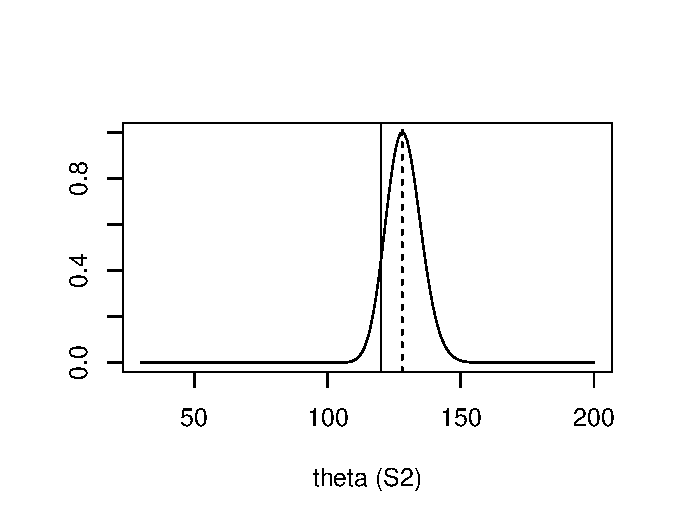
\includegraphics[width=0.49\textwidth]{fig/pod_likelihoodProf.pdf}
 \caption{An example of a likelihood profile for some $\theta$ estimate (vertival dashed line)
 using 30,000 samples drawn from a network of random variables, with $\theta=120$ (vertical
 solid line) for the $S1$ stage.} \label{fig:llprof}
\end{figure}

Moreover, the \code{logLikelihood} can then also be used to profile the likelihood (compare Figure
\ref{fig:llprof}) given the data to obtain confidence intervals for the parameter estimate. There
the true value of $\theta=120$ is shown as a solid vertical line and the estimate as the dashed
vertical line. 